% ------------------------------------------------------------------------------
% Chapter 1
% Delete this content and replace it with your own
% ------------------------------------------------------------------------------
\chapter{Markov Chains} % enter the name of the chapter here
\label{cha:markov-chains} % enter the chapter label here (for cross-referencing)

In this section, we shall understand what Markov Chain does. But before we move with the main topic of our dissertation, let us understand why Markov Chains are as a concept and which problems they solve. Markov Chains is a stochastic statistical process, which derive usage from probabilities of occurrences of different events. Now these events can either be independent or dependent, and overall probabilities shall still be calculated based on the frequency within the provided data. Then that data can be used to perform additional classification work on a sample testing dataset.

However, a \textbf{stochastic process} is defined as follows:

\vspace*{\fill} 
\begin{quote}
\centering 
\textit{In probability theory and related fields, a stochastic or random process is a mathematical object usually defined as a family of random variables. Stochastic processes are widely used as mathematical models of systems and phenomena that appear to vary in a random manner.}
\end{quote}
\vspace*{\fill}

Next section, we shall go over the basic properties of a Markov Chain structure and its corresponding model.

\begin{itemize}
    \item The probabilities of moving from a state to all others sum to one, 
    \item The probabilities apply to all system participants, and 
    \item The probabilities are constant over time
\end{itemize}

\section{Markov Assumption} % enter the name of the section here
\label{sec:markov-assumption} % enter the section label here (for cross referencing)

In probability theory, Markov property refers to memory-less property of a stochastic process. The latter has the Markov property if the probability distribution of future states of the process conditioned on both the past and present states depends only on the present state. In other words, predicting the next word in a sentence depends only on the current word, and not on the words that came before the current word. Markov property holds in a model if the values in any state are influenced only by the values of the immediately preceding or a small number of immediately preceding states. The hidden Markov model (HMM) is an example in which it is assumed that the Markov property holds.

In general language, a model is an imitation of a real-world scenario.  Models allow us to try to understand and predict what might happen in the real world in a low-risk, cost-effective and fast way. For example, in order to predict how Amazon can ship its products in the most cost-effective ways, models are run in order to design routes and ensure minimal costs are incurred, thus optimizing these routes. 

An important distinction is between deterministic models and random models. Another word for a random model is a stochastic model. Deterministic models do not contain any random components, so the output is completely determined by the inputs and any parameters. Random models have variable outcomes to account for uncertainty and unpredictability, so they can be run many times to give a sense of the range of possible outcomes. 

\subsection{Stochastic Processes} %enter the name of the subsection here
\label{sec:stochastic-processes} % enter the subsection label here (for cross-referencing)

A stochastic process, which we will usually write as  $X_{n}$, is an indexed sequence of random variables that are usually dependent on each other. Now, $X_{n}$ consists of random variables which take a value within a \textbf{State Space} S. A state space can be either discrete or continuous and a discrete state space corresponds to a set of distinct outcomes which can be finite or infinite. A state space is nothing but a list of all possible values for a given event. Now the State Space S can be either discrete or continuous, depending on what the variable looks like. For our topic of the dissertation, we shall be focusing on novel textual data, thus our sample space or state space shall be characters ranging from $A-Z, a-z, 0-9$ or special characters. 

Furthermore, a stochastic process can be broken down into an Index Set, which brings in a time variable, providing some order to the entire process of indexing. This helps us make the entire process measurable over time. Thus, time can sometimes be selected as discrete intervals or continuous. A stochastic or 'random' process can be defined as four distinct processes based on \textbf{State Space} and \textbf{Index Set}.

\begin{itemize}
    \item \textbf{Discrete Time, Discrete Space} \\
    A major example of this shall be the number of students attending a maths lecture.
    \textbf{Markov Chains} is a perfect example of how discrete time and discrete space work in practice. Each node has a value, a weightage, and multiple yet finite edges based on a simple model.
    \item \textbf{Discrete Time, Continuous Space} \\
    Daily maximum temperature can be a good example of discrete time, which is one day, and continuous space, where the variables can take any value.
    \item \textbf{Continuous Time, Discrete Space} \\
    The number of visitors on a page over time, where total visitors vary over a defined number and time is continuous.
    \item \textbf{Continuous Time, Continuous Space} \\
    Levels of a share index, where values continue to fluctuate and generally do not remain in a defined discrete space of the shares of any company.
\end{itemize}

\begin{figure}[H]
	\begin{center}
		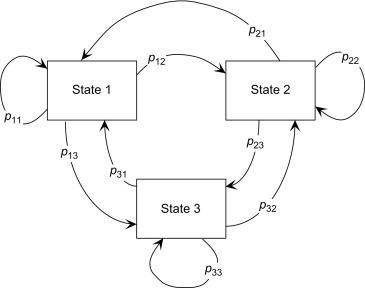
\includegraphics[width = 0.7\textwidth]{Images/markov_chain.jpg} % enter the filename here
		\caption{A simple example of states with discrete time.}
		\label{fig:markov-chain-state-space}
	\end{center}
\end{figure}

These Discrete Time Markov Chains are also what we shall be implementing in our novel classification problem further in the dissertation. We shall be focusing on a Discrete Space structure as part of the values. 

\section{Markov Property}
\label{sec:markov-property}
\textit{A stochastic process} $X = \left(X_{j}\right)_{j \in N_{0}}$ \textit{with values in a set space \textbf{S} is a Markov Chain if the following condition is met}.

\begin{equ}[!ht]
    \begin{equation}
    \begin{split}
        \label{eq:markov-chain-prop1}
        P \left( X_{j} \in A_{j} | X_{j-1} \in A_{j-1}, X_{j-2} \in A_{j-2}, \cdots, X_{0} \in A_{0} \right) \\ 
        &= P \left( X_{j} \in A_{j} | X_{j-1} \in A_{j-1} \right)
    \end{split}
    \end{equation}
\caption{\textit{$\forall A_0, A_1, \cdots, A_j \subseteq S$ and $j \in \mathbb{N}$}}
\end{equ}

This property works if the probability distribution $X_{j}$ depends on $X_{0}, \cdots, X_{j-2}$ through to $X_{j-1}$. And S is nothing but the state space or the sample space for the occurrence $\forall$ A. 

Now, let us try and demonstrate this property of Markov Chains through 2 simple examples.

\textbf{Example 1}: 
Let us denote $\left(\epsilon_{j}\right)_{j \in N_{0}}$ as identical independently distributed, i.e., i.i.d. random set of variables. The process X takes an assumption that $X_{0}$ = 0 and $X_j = X_{j-1} + \epsilon_j$, $\forall j \in \mathbb{N}$. If these conditions are satisfied, we can assume the model is a Markov Chain. And hence, we can denote $X_j$ as:
\begin{equ}[!ht]
    \begin{equation}
    \begin{split}
        \label{eq:markov-chain-prop1-ex1}
        X_j = \sum_{i = 1}^{j} \epsilon_{i}.
    \end{split}
    \end{equation}
\caption{In general, a Markov Chain is a random walk with some special cases.}
\end{equ}

\textbf{Example 2}: 
Let us denote $\left(\epsilon_{j}\right)_{j \in N_{0}}$ as identical independently distributed, i.e., i.i.d. random set of variables and this time, we have a variance of $Var\left(\epsilon_{j}\right)$ = 1. Then, this process can be given by $X_0$ = $X_1$ = 0 as the variance remains the same.

\begin{equ}[!ht]
    \begin{equation}
    \begin{split}
        \label{eq:markov-chain-prop1-ex2}
        X_{j} &= \frac{X_{j-1} + X_{j-2}}{2} + \epsilon_{j}
    \end{split}
    \end{equation}
\caption{And thus, $\forall$ j = 2,3,$\cdots$ is not a Markov Chain}.
\end{equ}

In the next two sections, we shall understand how the above Markov Property is useful when we distinguish between Discrete State Space Markov Chains and Continuous State Space Markov Chains.

\subsection{Discrete Space Markov Chains}
\label{sec:discrete-space-markov-chains}

In general working, when the state space is finite, such as for example, S = {1, 2, ..., N}, then the transition probabilities $P\left(X_{n} \in A_{n} | X_{n-1} \in A_{n-1}\right)$ in the equation \ref{eq:markov-chain-prop1} can be denoted with probabilities given by a short formula as 

\begin{equ}[!ht]
    \begin{equation}
    \begin{split}
        \label{eq:discrete-space-probdistro}
        p_{xy} = P \left( X_{j} = y | X_{j-1} = x \right)
    \end{split}
    \end{equation}
\caption{This equation is valid for all element pairs x, y $\in S$}.
\end{equ}

The resulting matrix P, which is derived by inserting values of the element pairs derived from the equation \ref{eq:discrete-space-probdistro}, i.e., $p_{xy}$ is known as the transition matrix. It would end up looking like this.

\begin{equ}[!ht]
    \begin{equation}
    \begin{split}
        \label{eq:discrete-time-transition-matrix}
        P = \left(
        \begin{array}{cccc}
        p_{11} & p_{12} & p_{13} & \cdots \\
        p_{21} & p_{22} & p_{23} & \cdots \\
        p_{31} & p_{32} & p_{33} & \cdots \\
        \vdots & \vdots & \vdots & \ddots
        \end{array}
        \right)
    \end{split}
    \end{equation}
\caption{This is how the transition matrix would be defined based on the number of variables we have}.
\end{equ}

When designing this transition probability matrix, we generally store a pair-mapping of each of the random variables and store their probability of occurrences. We shall see further that Markov Chains and Probability Matrices have a very deep relationship, as each distinct node can easily be considered a row and column value of this matrix. 
As an example, when we deal with characters as nodes in a Markov model, $p_{11}$ can be re-written as $p_{AA}$ if A is the first node of the model. It is pretty interchangeable but it can be simply explained as considering numerical numbers as an active denotation to simplify processes.

The matrix we considered is a finite one with limited variables. However, this transition matrix also works if we have an infinite state space and in those cases, our matrix P goes infinite as well. Now Discrete Markov Chains have a few Lemmas, which are important to keep in mind. Markov chains with finite or countably infinite state space are called Markov chains with \textit{discrete state space}.

\textbf{All of the following Lemmas are being taken from the book published by the Dr. Jochen Voss's taught module at the University of Leeds, and mentioned in their book, \textcite{voss:2013}}.

\subsubsection{Lemma 1}
\label{sec:discrete-markov-prop1}
Let $P^{SxS}$ be the transition matrix of a Markov Chain with state space, S. Then $P = \left(p_{xy}\right)_{x, y \in S}$ has the following properties:

\begin{enumerate}
    \item $p_{xy} \geq 0$ which stands true $\forall x, y \in S$.
    \item $\sum_{y \in S} p_{xy} = 1$ which stands true $\forall x \in S$. 
\end{enumerate}

A matrix that satisfies both the above conditions is known as a \textbf{stochastic matrix}. Additionally, a vector $\pi \in \mathbb{R}_{S}$ is called a probability vector, if $\pi_{x} \geq 0$ $\forall x \in S$ and $\sum_{x \in S} \pi_{x} = 1$. 

As we shall see in a later section, in order to simulate a Markov Chain, we shall require an input probability matrix $\pi$, and a transition matrix P, already defined to define any transition probabilities. For reference, the probability vector we shall be using is the probability of a novel occurring in a text and our probability of a character occurring in a novel would constitute the transition matrix.

\subsubsection{Lemma 2}
\label{sec:discrete-markov-prop2}

Let X be a time-homogeneous Markov chain with finite state space, and a transition matrix P. Then
\begin{equ}[!ht]
    \begin{equation}
    \begin{split}
        \label{eq:markov-discrete-lemma2}
        P \left( X_{j+k} = y | X_{j} = x \right) = \left( P^k \right)_{xy}
    \end{split}
    \end{equation}
\caption{$\forall j, k \in \mathbb{N}_{0}$ and $x, y \in S$, where $P^k = P. P \cdots P$ is the kth power of the transition matrix P}.
\end{equ}

Now we shall go about proving this lemma. That is important as need to figure out why time-homogeneous Markov chains function. 
\textbf{Proof}: For k = 0, the matrix $P^{0}$ is by definition the identity matrix and the statement
holds. Also, for k = 1 we have

\begin{equ}[!ht]
    \begin{equation}
    \begin{split}
        \label{eq:markov-discrete-lemma2-proof1}
        P \left( X_{j+1} = y | X_{j} = x \right) = p_{xy} = \left( P^1 \right)_{xy}
    \end{split}
    \end{equation}
\caption{by the definition of the transition matrix from equation \ref{eq:discrete-time-transition-matrix}}.
\end{equ}

Now we assume k $>$ 1 and the statement holds true for k-1, then we have

\begin{equ}[H]
    \begin{equation}
    \begin{split}
        \label{eq:markov-discrete-lemma2-proof2}
        P \left(X_{j+k} = y | X_{j} = x \right) \\
        &= \frac{P \left(X_{j+k} = y, X_{j} = x \right)}{P \left(X_{j} = x \right)} \\
        &= \frac{1}{P \left(X_{j} = x \right)} \sum_{z \in S} P \left(X_{j+k} = y, X_{j+k-1} = z, X_{j} = x \right) \\
        &= \frac{1}{P \left(X_{j} = x \right)} \sum_{z \in S} P \left(X_{j+k-1} = z, X_{j} = x \right) \\ &. P \left(X_{j+k} = y | X_{j+k-1} = z, X_{j} = x \right)  \\
    \end{split}
    \end{equation}
\caption{extended from the previous equation \ref{eq:markov-discrete-lemma2-proof1}}.
\end{equ}

Thus, using the Markov chain property from \ref{eq:markov-chain-prop1}, we use that property with this equation \ref{eq:markov-discrete-lemma2-proof2}

\begin{equ}[!ht]
    \begin{equation}
    \begin{split}
        \label{eq:markov-discrete-lemma2-proof3}
        P \left(X_{j+k} = y | X_{j} = x \right) \\
        &= \sum_{z \in S} \frac{P \left(X_{j+k-1} = z | X_{j} = x \right)}{P \left(X_{j} = x \right)} \\
        &= \sum_{z \in S} P \left(X_{j+k-1} = z | X_{j} = x \right) p_{xy} \\
        &= \sum_{z \in S} \left( P^{k-1} \right)_{xy} p_{xy}. 
    \end{split}
    \end{equation}
\caption{The above equation is basically a matrix-matrix multiplication of $P^{k-1}$ and $P$ probability transition matrices}.
\end{equ}

Now after we perform the matrix-matrix multiplication, we get the final equation of the Lemma 2.

\begin{equ}[!ht]
    \begin{equation}
    \begin{split}
        \label{eq:markov-discrete-lemma2-proof5}
        P \left(X_{j+k} = y | X_{j} = x \right) = \left( P^{k-1} . P\right)_{xy} = \left( P^{k} \right)_{xy}
    \end{split}
    \end{equation}
\caption{And we can summarize the lemma 2 using this equation above.}
\end{equ}


\subsubsection{Lemma 3}
\label{sec:discrete-markov-prop3}

Let X be a time-homogeneous Markov chain with finite state space and a transition state P and initial distribution $\pi$. Then we have 

\begin{equ}[!ht]
    \begin{equation}
    \begin{split}
        \label{eq:markov-discrete-lemma3}
        P \left(X_{j} = y\right) = \left(\pi^{T} P^{j}\right)_{y}
    \end{split}
    \end{equation}
\caption{$\forall y \in S$ }
\end{equ}

Now we shall go about proving this Lemma.

\textbf{Proof}: At time 0, the equation \ref{eq:markov-discrete-lemma3} can be reduced to

\begin{equ}[!ht]
    \begin{equation}
    \begin{split}
        \label{eq:markov-discrete-lemma3-proof1}
        P\left(X_{0} = x\right) = \pi_{x}
    \end{split}
    \end{equation}
\caption{$\forall x \in S$ }
\end{equ}

For time k $>$ 0, we can use Bayes' formula to come up with a summary as follows:

\begin{equ}[!ht]
    \begin{equation}
    \begin{split}
        \label{eq:markov-discrete-lemma3-proof2}
        P \left(X_{j} = y\right) = \sum_{x \in S} P \left(X_{j} = y | X_{0} = x\right) \\
        &= \sum_{x \in S} P \left(X_{0} = x\right) P \left(X_{j} = y | X_{0} = x\right) \\
        &= \sum_{x \in S} \pi_{x} \left( P^{j}\right)_{xy}
    \end{split}
    \end{equation}
\caption{$\forall y \in S$ }
\end{equ}

We need to consider a transposed vector $\pi^{T}$ as a matrix with one row and S columns, the equation \ref{eq:markov-discrete-lemma3-proof2} can be written as a matrix-matrix multiplication. 
Since X is a time-homogeneous Markov chain with a transition matrix, P. A probability matrix $\pi$ is called a \textit{stationary distribution} of X if $\pi^{T}.P = \pi^{T}$, leads us to the equation

\begin{equ}[!ht]
    \begin{equation}
    \begin{split}
        \label{eq:markov-discrete-lemma3-proof3}
        \sum_{x \in S} \pi_{x} p_{xy} = \pi_{y}
    \end{split}
    \end{equation}
\caption{$\forall y \in S$ }
\end{equ}

Now through the equation \ref{eq:markov-discrete-lemma3-proof1}, we already know that 

\begin{equ}[!ht]
    \begin{equation}
    \begin{split}
        \label{eq:markov-discrete-lemma3-proof4}
        P \left(X_{j} = y\right) = \left( \pi^{T} P^{j}\right)_{y}
    \end{split}
    \end{equation}
\caption{$\forall y \in S$ }
\end{equ}

\subsection{Continuous Space Markov Chains}

Even though we shall not be using continuous Markov chains for the purposes of our dissertation, we shall briefly understand what continuous Markov chains look like and go over their structure, how to incorporate them through an algorithm and take an example.

Markov chains can be considered on very general state spaces, but here we restrict ourselves to the case $S = \mathbb{R}^{d}$ . Most of the results from the previous section formally carry over to the case of continuous state space, with only changes in notation. Now instead of an infinite transition matrix P, we shall be using transition kernels which will be defined below.

A \textit{transition kernel} is a map $P\left(.,.\right)$ such that:

\begin{enumerate}
    \item $P \left(x, A\right) \geq 0$ for all $x \subseteq \mathbb{R}^{d}$ and all $A \subseteq {R}^{d}$; and 
    \item $P \left(x, .\right)$ is a probability distribution on $\mathbb{R}^{d}$ for all $x \in \mathbb{R}^{d}$.
\end{enumerate}

The idea behind a transition kernel is that it is a map of the distribution of the next value of the Markov chain. Keeping in mind that a continuous state space would tentatively have infinite values, a map would be the best idea to denote what the transition state could look like. Now, the map A $\rightarrow$ $P \left(x, A\right)$ is denoted as the distribution of the subsequent Markov chain. And hence, we can define the transition kernel with one equation below.

\begin{equ}[!ht]
    \begin{equation}
    \begin{split}
        \label{eq:markov-continuous-transition-kernel}
        P \left(x, A\right) = P \left(X_{j} \in A | X_{j-1} = x\right).
    \end{split}
    \end{equation}
\end{equ}

Additionally, there is a topic named transition density which comes into factor when dealing with continuous variables. Thus, if X is a Markov chain then the transition density is described as follows.

\begin{equ}[!ht]
    \begin{equation}
    \begin{split}
        \label{eq:markov-continuous-transition-density}
        P \left(X_{j} \in A | X_{j-1} = x\right) = \int_{A} p \left(x, y\right) dy
    \end{split}
    \end{equation}
    \caption{$\forall x \in \mathbb{R}^{d}$}
\end{equ}



\textbf{Algorithm of Markov chains with continuous state space} \\
Input: \\
A probability density π: Rd → [0,$\infty$) \\
A transition density p: Rd × Rd → [0,$\infty$) \\
Randomness used: \\
One sample $X_{0} \sim \pi$ \\
Samples from the densities $p \left(x, .\right)$ for $x \in \mathbb{R}$ \\
Output: \\
A path of a Markov chain with initial distribution $\pi$ and transition matrix P \\
1: Generate $X_{0} \sim \pi$ \\
2: Output $X_{0}$ \\
3: For $j = 1, 2, 3, \cdots $ \textbf{do} \\
4: Generate $X_{j} \sim$ $p \left( X_{j-1}, . \right)$ \\
5: Output $X_{j}$ \\
6: End for

This is the algorithm we would use to implement a continuous state Markov model. \\


\section{Markov Chain Example}

Now, we shall go over a sample example of a completely interconnected 3-state Markov Chain. When we solve for a Markov Chain, we try to solve for when all the states would return 1 as their final solution. 

\begin{figure}[htb]
\label{fig:markov-chain-example-1}
\centering
\begin{tikzpicture}
\node[state, align = center] (s1) {State 1};
\node[state, below right of=s1]  (s2) {State 2};
\node[state, below left of=s1] (s3) {State 3};

\draw (s1) edge[loop above] node {$1/4$} (s1);
\draw (s1) edge[bend left] node {$1/2$} (s2);
\draw (s1) edge[bend left=12] node {$1/4$} (s3);

\draw (s2) edge[bend left=12] node {$2/3$} (s1);
\draw (s2) edge[loop right] node {$1/6$} (s2);
\draw (s2) edge[bend right=12] node {$1/6$} (s3);

\draw (s3) edge[bend left] node {$1/6$} (s1);
\draw (s3) edge[bend right] node {$1/2$} (s2);
\draw (s3) edge[loop left] node {$1/3$} (s3);

\end{tikzpicture}
\caption{Example 1 of a 3-State Markov Chain}
\end{figure}

Therefore, the Transition Matrix of this completely interconnected Markov Model is denoted by:

\begin{equ}[!ht]
    \begin{equation}
    \begin{split}
        \label{eq:markov-chain-ex1}
        P = \left(
        \begin{array}{ccc}
        1/4 & 1/2 & 1/4 \\
        2/3 & 1/6 & 1/6 \\
        1/6 & 1/2 & 1/3
        \end{array}
        \right)
    \end{split}
    \end{equation}
\caption{Transition Matrix 1}.
\end{equ}

Similarly, if a few certain nodes end up missing, further is a second example:

\begin{figure}[htb]
\label{fig:markov-chain-example-2}
\centering
\begin{tikzpicture}
\node[state, align = center] (s1) {State 1};
\node[state, below right of=s1]  (s2) {State 2};
\node[state, below left of=s1] (s3) {State 3};

\draw (s1) edge[loop above] node {$3/4$} (s1);
\draw (s1) edge[bend left] node {$1/4$} (s2);
%\draw (s1) edge[bend left=12] node {$1/4$} (s3);

\draw (s2) edge[bend left=12] node {$2/3$} (s1);
%\draw (s2) edge[loop right] node {$1/6$} (s2);
\draw (s2) edge[bend right=12] node {$1/3$} (s3);

\draw (s3) edge[bend left] node {$1/6$} (s1);
\draw (s3) edge[bend right] node {$1/2$} (s2);
\draw (s3) edge[loop left] node {$1/3$} (s3);

\end{tikzpicture}
\caption{Example 2 of a 3-State Markov Chain}
\end{figure}

Therefore, the Transition Matrix of this completely interconnected Markov Model is denoted by:

\begin{equ}[!ht]
    \begin{equation}
    \begin{split}
        \label{eq:markov-chain-ex2}
        P = \left(
        \begin{array}{ccc}
        1/4 & 1/2 & 1/4 \\
        2/3 & 1/6 & 1/6 \\
        1/6 & 1/2 & 1/3
        \end{array}
        \right)
    \end{split}
    \end{equation}
\caption{Transition Matrix 2}.
\end{equ}